\documentclass[10pt,a4paper,twocolumn]{article}

\usepackage[margin=2cm]{geometry}
\usepackage{graphicx}
\usepackage{amsmath,amssymb}
\usepackage{hyperref}
\usepackage{natbib}
\usepackage{booktabs}
\usepackage{url}
\usepackage{enumitem}
\usepackage{xcolor}
\usepackage{float}
\usepackage{caption}
\usepackage{titlesec}
\usepackage{tikz}
\usetikzlibrary{shapes.geometric, arrows.meta, positioning, fit, backgrounds, calc}

\hypersetup{colorlinks=true, linkcolor=blue!60!black, citecolor=blue!60!black, urlcolor=blue!60!black}
\titleformat{\section}{\large\bfseries}{\thesection.}{0.5em}{}
\titleformat{\subsection}{\normalsize\bfseries}{\thesubsection}{0.5em}{}
\setlength{\parskip}{0.3em}

\title{\textbf{A Survey of Deep Learning-Based Reconstruction Methods\\for Quantum Imaging Systems}}

\author{
Oishik Kar\\
\small Department of Computer Science and Engineering\\
\small Indian Institute of Information Technology Dharwad\\
\small \texttt{23bcs089@iiitdwd.ac.in}
}

\date{June 2026 \quad\textbar\quad PARIMANA Summer Internship Program, Qmet Tech Foundation}

\begin{document}

\twocolumn[
\maketitle

\begin{center}
\begin{minipage}{0.92\textwidth}
\textbf{Abstract.}
Quantum imaging systems, including ghost imaging, entangled-photon compressed sensing, and sub-shot-noise microscopy, exploit non-classical photon correlations to surpass classical limits in sensitivity and resolution. However, reconstructing high-quality images from the sparse, noisy measurements intrinsic to these systems remains computationally demanding. This survey reviews deep learning architectures applied to quantum imaging reconstruction. We categorise methods along three axes: imaging modality, neural network architecture, and reconstruction task. Our review shows that deep learning enables measurement reductions of one to two orders of magnitude in ghost imaging, identifies a convergence towards U-Net and GAN-based architectures, and highlights critical gaps in standardised benchmarking. We conclude by discussing hybrid classical--quantum reconstruction frameworks and proposing directions for quantum-inspired neural architectures in imaging pipelines.

\vspace{0.5em}
\noindent\textbf{Keywords:} quantum imaging, ghost imaging, deep learning, compressed sensing, image reconstruction, quantum optics, neural networks
\end{minipage}
\end{center}
\vspace{0.8em}
]

\section{Introduction}
\label{sec:introduction}

Quantum imaging harnesses the non-classical correlations of entangled or correlated photon pairs to achieve imaging modalities that are not accessible with classical light sources. Since the seminal demonstration of imaging via two-photon entanglement by \citet{pittman1995}, the field has expanded to encompass ghost imaging, quantum illumination, sub-shot-noise microscopy, and entanglement-assisted compressed sensing. These techniques promise advantages in spatial resolution, noise robustness, and the ability to image with photons that never interact with the object \citep{erkmen2010}.

Despite these capabilities, a key challenge remains: \emph{image reconstruction}. Quantum imaging measurements are inherently sparse, limited by detector efficiencies, coincidence counting rates, and photon budgets, and the resulting inverse problems are severely ill-posed. Traditional reconstruction approaches rely on correlation computation or iterative optimisation, which demand large numbers of measurements and significant computation time.

Deep learning has proved effective for solving inverse problems in computational imaging \citep{barbastathis2019, lecun2015} and is now being applied to quantum imaging reconstruction. Neural networks can learn strong image priors from data, enabling high-quality reconstruction from far fewer measurements than classical algorithms require. Work at the intersection of quantum optics and deep learning now spans multiple imaging modalities and network architectures.

\subsection{Scope and Contributions}

This survey provides a systematic review of deep learning methods applied to quantum imaging reconstruction. We focus on three principal modalities:

\begin{enumerate}[label=(\roman*)]
    \item \textbf{Quantum ghost imaging}, where deep learning dramatically reduces measurement requirements for image reconstruction from spatially correlated photon fields.
    \item \textbf{Compressed sensing with quantum correlations}, where neural networks enhance reconstruction from sub-Nyquist quantum measurements.
    \item \textbf{Sub-shot-noise imaging}, where deep learning denoising exploits quantum noise statistics to push sensitivity below the classical shot-noise limit.
\end{enumerate}

The contributions of this survey are:
\begin{itemize}
    \item A unified taxonomic framework classifying methods by imaging modality, DL architecture, and reconstruction task.
    \item A detailed comparative analysis of deep learning approaches for ghost imaging reconstruction, including quantitative performance comparisons.
    \item Identification of critical gaps in benchmarking, reproducibility, and standardisation.
    \item A discussion of hybrid classical--quantum architectures and future research directions.
\end{itemize}

\noindent Figure~\ref{fig:taxonomy} illustrates this classification framework.

\begin{figure*}[t]
\centering
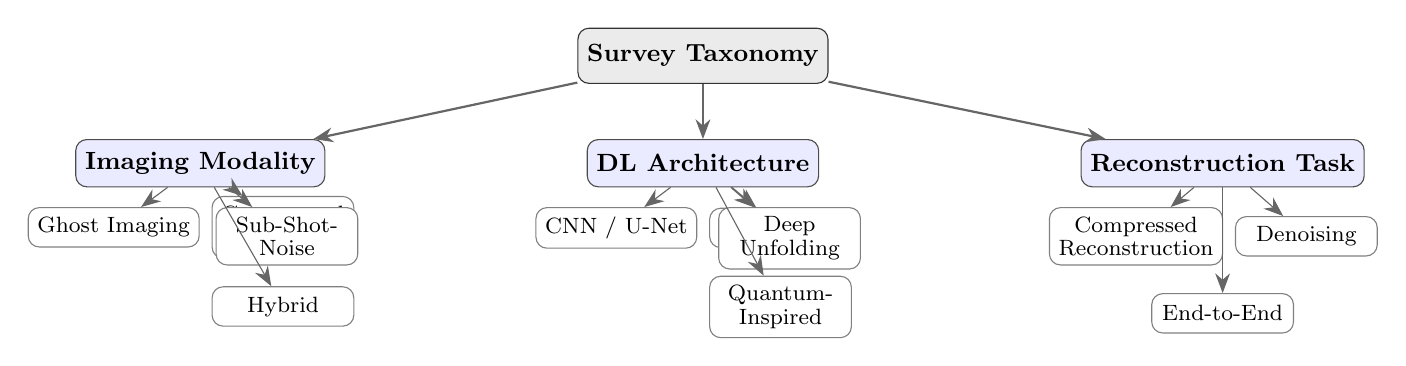
\begin{tikzpicture}[
    node distance=0.4cm and 0.6cm,
    rootnode/.style={rectangle, rounded corners, draw=black!80, fill=black!8, font=\bfseries\small, minimum height=0.7cm, minimum width=2.8cm, align=center},
    axisnode/.style={rectangle, rounded corners, draw=black!70, fill=blue!8, font=\small\bfseries, minimum height=0.6cm, minimum width=2.2cm, align=center},
    leafnode/.style={rectangle, rounded corners, draw=black!50, fill=white, font=\footnotesize, minimum height=0.5cm, minimum width=1.8cm, align=center},
    arr/.style={-{Stealth[length=2.5mm]}, thick, black!60}
]

% Root
\node[rootnode] (root) {Survey Taxonomy};

% Three axes
\node[axisnode, below left=0.7cm and 3.2cm of root] (mod) {Imaging Modality};
\node[axisnode, below=0.7cm of root] (arch) {DL Architecture};
\node[axisnode, below right=0.7cm and 3.2cm of root] (task) {Reconstruction Task};

\draw[arr] (root) -- (mod);
\draw[arr] (root) -- (arch);
\draw[arr] (root) -- (task);

% Modality leaves
\node[leafnode, below=0.25cm of mod, xshift=-1.1cm] (m1) {Ghost Imaging};
\node[leafnode, right=0.15cm of m1] (m2) {Compressed\\[-1pt]Sensing};
\node[leafnode, below=0.25cm of mod, xshift=1.1cm] (m3) {Sub-Shot-\\[-1pt]Noise};
\node[leafnode, below=0.35cm of m2] (m4) {Hybrid};

\draw[arr, thin] (mod) -- (m1);
\draw[arr, thin] (mod) -- (m2);
\draw[arr, thin] (mod) -- (m3);
\draw[arr, thin] (mod) -- (m4);

% Architecture leaves
\node[leafnode, below=0.25cm of arch, xshift=-1.1cm] (a1) {CNN / U-Net};
\node[leafnode, right=0.15cm of a1] (a2) {GAN};
\node[leafnode, below=0.25cm of arch, xshift=1.1cm] (a3) {Deep\\[-1pt]Unfolding};
\node[leafnode, below=0.35cm of a2] (a4) {Quantum-\\[-1pt]Inspired};

\draw[arr, thin] (arch) -- (a1);
\draw[arr, thin] (arch) -- (a2);
\draw[arr, thin] (arch) -- (a3);
\draw[arr, thin] (arch) -- (a4);

% Task leaves
\node[leafnode, below=0.25cm of task, xshift=-1.1cm] (t1) {Compressed\\[-1pt]Reconstruction};
\node[leafnode, right=0.15cm of t1] (t2) {Denoising};
\node[leafnode, below=0.35cm of t1, xshift=1.1cm] (t3) {End-to-End};

\draw[arr, thin] (task) -- (t1);
\draw[arr, thin] (task) -- (t2);
\draw[arr, thin] (task) -- (t3);

\end{tikzpicture}
\caption{Taxonomic classification framework used in this survey. Methods are categorised along three axes: the quantum imaging modality, the deep learning architecture, and the reconstruction task.}
\label{fig:taxonomy}
\end{figure*}

\subsection{Paper Organisation}

Section~\ref{sec:background} reviews the necessary background in quantum imaging and deep learning for inverse problems. Section~\ref{sec:ghost_imaging} surveys deep learning methods for ghost imaging in detail. Section~\ref{sec:compressed_sensing} covers compressed sensing with quantum correlations. Section~\ref{sec:sub_shot_noise} addresses sub-shot-noise imaging. Section~\ref{sec:hybrid} examines hybrid classical--quantum architectures. Section~\ref{sec:discussion} discusses open problems, and Section~\ref{sec:conclusion} concludes.

\section{Background}
\label{sec:background}

\subsection{Quantum Imaging Fundamentals}

Quantum imaging relies on photon pairs generated through spontaneous parametric down-conversion (SPDC), in which a pump photon incident on a nonlinear crystal produces two daughter photons---conventionally termed \emph{signal} and \emph{idler}---that are correlated in position, momentum, and time. These correlations arise from the phase-matching conditions of the nonlinear interaction and can be either classical or genuinely quantum (entangled) depending on the experimental configuration.

The spatial correlations between signal and idler photons enable imaging protocols where information about an object is extracted by measuring correlations between spatially separated detectors, rather than by direct imaging. This principle underlies ghost imaging, quantum illumination, and related protocols.

\subsection{Ghost Imaging: From Quantum to Computational}

Ghost imaging (GI) was first demonstrated by \citet{pittman1995} using entangled photon pairs from SPDC. In the original configuration, the object is placed in the path of one photon (say, the signal), which is detected by a single-pixel (bucket) detector that records no spatial information. The partner idler photon, which never interacts with the object, is detected by a spatially resolving detector. Individually, neither detector's output contains an image; the image emerges only from the \emph{coincidence} correlations between the two detectors.

The quantum nature of the original ghost imaging was debated after \citet{bennink2002} demonstrated a similar effect using classically correlated thermal light, and \citet{ferri2005} achieved high-resolution ghost imaging with pseudothermal sources. \citet{shapiro2008} subsequently introduced \emph{computational} ghost imaging (CGI), in which the spatially resolving detector is replaced entirely by computational knowledge of the illumination patterns. In CGI, a spatial light modulator generates known random patterns, the object is illuminated by each pattern in sequence, and a bucket detector records the total transmitted intensity. The image is reconstructed by correlating the known patterns with the bucket detector readings:

\begin{equation}
    I(\mathbf{r}) = \frac{1}{M} \sum_{m=1}^{M} \left( B_m - \langle B \rangle \right) \phi_m(\mathbf{r}),
    \label{eq:gi_correlation}
\end{equation}

\noindent where $B_m$ is the bucket detector signal for the $m$-th pattern $\phi_m(\mathbf{r})$, $\langle B \rangle$ is the mean bucket signal, and $M$ is the total number of measurements. High-quality reconstruction via Eq.~\eqref{eq:gi_correlation} typically requires $M$ to be comparable to or greater than the number of pixels in the reconstructed image \citep{erkmen2010}, motivating the development of more efficient reconstruction methods.

\subsection{Deep Learning for Inverse Problems}

Deep learning has emerged as a dominant paradigm for solving inverse problems in imaging, where the goal is to recover a signal $\mathbf{x}$ from measurements $\mathbf{y} = \mathcal{A}(\mathbf{x}) + \mathbf{n}$, with $\mathcal{A}$ denoting the forward measurement operator and $\mathbf{n}$ representing noise \citep{barbastathis2019}.

Several architecture families are particularly relevant to quantum imaging. Convolutional neural networks (CNNs) learn hierarchical spatial features through convolutional filters, enabling effective image-to-image mappings for denoising and reconstruction \citep{lecun2015}. The U-Net architecture \citep{ronneberger2015} extends the convolutional approach with an encoder--decoder structure and skip connections that preserve fine-grained spatial information, and has been widely adopted for biomedical and computational imaging tasks. Generative adversarial networks (GANs) employ a generator--discriminator framework that produces perceptually realistic reconstructions by learning the distribution of natural images \citep{goodfellow2014}. Autoencoders, which learn compressed latent representations from which images can be reconstructed, are also relevant for dimensionality reduction in quantum measurement data.

\citet{barbastathis2019} provide a comprehensive review of deep learning for computational imaging, noting that learned approaches can outperform traditional iterative methods in both speed and quality, particularly when training data adequately represents the target image distribution.

\subsection{Compressed Sensing Theory}

Compressed sensing (CS) provides a mathematical framework for recovering sparse signals from sub-Nyquist measurements \citep{donoho2006, candes2006}. A signal $\mathbf{x} \in \mathbb{R}^n$ that is $k$-sparse in some basis $\Psi$ can be recovered from $m \ll n$ linear measurements $\mathbf{y} = \Phi \mathbf{x}$ if the measurement matrix $\Phi$ satisfies the restricted isometry property (RIP).

The relevance of CS to quantum imaging is twofold. First, quantum correlations can provide natural incoherence between measurement and sparsity bases, satisfying CS recovery conditions \citep{katz2009}. Second, the extreme photon scarcity in quantum imaging makes sub-Nyquist reconstruction practically essential. \citet{katz2009} demonstrated compressive ghost imaging, achieving image reconstruction with far fewer measurements than the Nyquist limit by exploiting image sparsity, and subsequent work has combined CS with deep learning to further improve reconstruction quality.

\section{Deep Learning for Ghost Imaging Reconstruction}
\label{sec:ghost_imaging}

The application of deep learning to ghost imaging reconstruction has been the most active area at the intersection of quantum imaging and neural networks. This section reviews the principal approaches, organised by network architecture.

\subsection{Fully Connected and CNN-Based Approaches}

\citet{lyu2017} provided the first demonstration that a neural network could reconstruct ghost images from bucket detector measurements. Their approach used a fully connected network trained on pairs of bucket signals and ground-truth images, achieving recognisable reconstruction of $28 \times 28$ handwritten digits at a sampling ratio as low as 12.5\%---a dramatic improvement over the correlation-based method (Eq.~\ref{eq:gi_correlation}), which requires sampling ratios approaching 100\% for comparable quality.

\citet{he2018} extended this work with a convolutional architecture, demonstrating improved generalisation to object categories not seen during training. Their CNN employed multiple convolutional layers with batch normalisation and ReLU activations, and was validated on both simulated and experimental ghost imaging data. Notably, the CNN-based approach maintained reasonable reconstruction quality even at sampling ratios below 10\%, where traditional methods produce severely degraded images.

\citet{shimobaba2018} applied deep learning specifically to computational ghost imaging, replacing the correlation computation of Eq.~\eqref{eq:gi_correlation} with a learned mapping. Their results confirmed that deep learning consistently outperforms traditional correlation-based reconstruction, particularly in low-measurement regimes.

\subsection{GAN-Based Reconstruction}

Generative adversarial networks \citep{goodfellow2014} have been applied to ghost imaging to improve the perceptual quality of reconstructions. The adversarial training framework encourages the generator to produce images that are statistically indistinguishable from real images, yielding reconstructions with sharper edges and more realistic textures than those obtained from MSE-trained networks.

However, GAN-based methods carry an inherent risk of \emph{hallucination}---generating plausible but incorrect image features---which is particularly concerning in scientific imaging applications where fidelity to the true object is paramount. This trade-off between perceptual quality and pixel-level accuracy remains an active area of investigation.

\subsection{End-to-End Learned Approaches}

A significant advance was made by \citet{wang2019}, who proposed jointly optimising the illumination patterns and the reconstruction network in an end-to-end differentiable framework. Rather than using random illumination patterns and learning only the reconstruction mapping, their approach learns \emph{optimal measurement strategies} tailored to the reconstruction network.

This end-to-end optimisation achieved 3--5\,dB improvement in PSNR over methods that separately optimise illumination and reconstruction, demonstrating that the measurement and reconstruction stages are fundamentally coupled and benefit from joint design. The approach also provides insight into what constitutes an ``informative'' measurement in the context of ghost imaging.

\subsection{Comparative Analysis}

Table~\ref{tab:gi_comparison} summarises the key characteristics and reported performance of the reviewed deep learning methods for ghost imaging reconstruction.

\begin{table*}[t]
\centering
\footnotesize
\caption{Comparison of deep learning methods for ghost imaging reconstruction.}
\label{tab:gi_comparison}
\begin{tabular}{@{}lp{2.2cm}cccl@{}}
\toprule
\textbf{Reference} & \textbf{Architecture} & \textbf{Size} & \textbf{Sampling} & \textbf{Data} & \textbf{Key Contribution} \\
\midrule
Lyu et al.\ [2017]       & Fully connected  & $28\times28$   & 12.5\%  & Sim.     & First DL-based ghost imaging reconstruction \\
He et al.\ [2018]        & CNN              & $28\times28$   & $<$10\% & Sim.+Exp. & Improved generalisation to unseen categories \\
Shimobaba et al.\ [2018] & CNN              & $64\times64$   & 25\%    & Sim.     & Applied DL to computational GI \\
Wang et al.\ [2019]      & End-to-end CNN   & $64\times64$   & 6.25\%  & Sim.     & Joint optimisation of patterns and network \\
\bottomrule
\end{tabular}
\end{table*}

Several trends emerge from this comparison. First, all methods achieve usable reconstruction quality at sampling ratios well below the Nyquist limit, confirming the strong regularising effect of learned image priors. Second, the field has progressed from simple fully connected architectures to more sophisticated end-to-end frameworks. Third, there is a notable lack of standardised benchmarks: different papers use different image sizes, datasets, noise models, and evaluation metrics, making rigorous cross-method comparison difficult.

\subsection{Discussion}

The reviewed works establish that deep learning is a transformative tool for ghost imaging reconstruction. However, several limitations persist. Most studies operate on small image sizes ($28\times28$ to $64\times64$); scalability to high-resolution imaging remains underexplored. The reliance on simulated data in many studies raises questions about robustness to real experimental noise and detector imperfections. Finally, the fundamental question of whether quantum correlations provide an advantage over classical correlations \emph{when combined with deep learning} has not been systematically addressed.

\section{Compressed Sensing with Quantum Correlations}
\label{sec:compressed_sensing}

Compressed sensing (CS) provides a natural framework for quantum imaging, where measurements are inherently limited by photon budgets and detector constraints. This section reviews the integration of deep learning with CS approaches that exploit quantum correlations.

\subsection{Quantum Compressed Sensing Fundamentals}

\citet{katz2009} demonstrated that ghost imaging can be formulated as a compressed sensing problem, achieving image reconstruction from significantly fewer measurements than the Nyquist limit by exploiting the sparsity of natural images. In this framework, the bucket detector measurements constitute the compressed observations $\mathbf{y} = \Phi \mathbf{x}$, where $\Phi$ is determined by the illumination patterns and $\mathbf{x}$ is the image to be recovered.

The quantum advantage in this context arises from two sources. First, entangled photon pairs can provide measurement matrices with favourable incoherence properties, naturally satisfying the conditions required for CS recovery \citep{donoho2006, candes2006}. Second, quantum correlations enable noise rejection through coincidence detection, effectively improving the signal-to-noise ratio of each measurement.

\subsection{Neural Network Enhanced CS Reconstruction}

% need to add: LISTA-type approaches, deep unfolding, data-driven vs model-based comparison

Traditional CS recovery algorithms (e.g., basis pursuit, iterative hard thresholding) are computationally expensive and require careful tuning of regularisation parameters. Deep learning offers two strategies for improvement: (i)~\emph{purely data-driven} approaches that learn a direct mapping from compressed measurements to images, bypassing explicit sparsity assumptions; and (ii)~\emph{deep unfolding} approaches that parameterise iterative CS algorithms as neural networks, combining the interpretability of model-based methods with the flexibility of learned parameters.

Both strategies have shown promise in classical compressed imaging and are beginning to be explored in the quantum setting, where the unique noise statistics of photon-counting measurements introduce additional challenges.

\subsection{Entanglement-Assisted Measurement Optimisation}

% expand -- connection to tomography, entangled probes for measurement design

An emerging direction explores the use of entangled photon states to design measurement bases that are optimally suited for compressed sensing recovery. This connects to the broader field of quantum state tomography, where similar compressed measurement strategies have been developed. The potential for deep learning to jointly optimise entangled measurement strategies and reconstruction networks---extending the end-to-end approach of \citet{wang2019} to the quantum domain---remains largely unexplored.

\section{Sub-Shot-Noise Imaging}
\label{sec:sub_shot_noise}

Sub-shot-noise imaging exploits quantum correlations between photon pairs to achieve sensitivity below the classical shot-noise limit, which bounds the minimum noise in measurements made with coherent (classical) light sources.

\subsection{Quantum Noise Limits in Imaging}

\citet{brida2010} provided the first experimental demonstration of sub-shot-noise quantum imaging, achieving a noise reduction of approximately 40\% below the shot-noise level using spatially entangled photon pairs from SPDC. \citet{samantaray2017} subsequently realised the first sub-shot-noise wide-field microscope, extending the technique from proof-of-concept to a practical imaging modality capable of operating over extended fields of view.

The quantum enhancement in these systems arises from the photon-number correlations between signal and idler beams: by subtracting the idler intensity from the signal, classical noise sources are suppressed below the shot-noise floor. However, the improvement is limited by optical losses and detector inefficiencies, which degrade the quantum correlations.

\subsection{Deep Learning Denoising for Quantum-Enhanced SNR}

% add: noise models (Poissonian vs sub-Poissonian), DL denoising archs, compare w/ BM3D/NLM

Deep learning denoising represents a promising direction for extending the practical advantage of sub-shot-noise imaging. Classical denoising algorithms assume Gaussian or Poissonian noise statistics, which do not accurately describe the sub-Poissonian noise in quantum-correlated imaging. Neural networks trained on data with appropriate quantum noise models could exploit the specific statistical structure of quantum measurements to achieve superior denoising performance.

Furthermore, deep learning may help compensate for the optical losses that currently limit practical sub-shot-noise imaging, effectively widening the parameter regime in which quantum advantage is achievable. This possibility has been explored in related contexts such as deep learning microscopy \citep{rivenson2017}, but dedicated studies in the quantum imaging setting remain sparse.

\section{Hybrid Classical--Quantum Architectures}
\label{sec:hybrid}

Recent work has explored hybrid architectures that combine classical neural network components with quantum-inspired or quantum-computational elements for imaging reconstruction. This section reviews tensor network approaches, variational quantum circuits, and the practical challenges of integrating quantum computation into imaging pipelines.

\subsection{Quantum-Inspired Neural Networks}

Tensor networks, originally developed for simulating quantum many-body systems, have been adapted for classical machine learning tasks including image classification. \citet{stoudenmire2016} demonstrated that matrix product states (MPS), a one-dimensional tensor network ansatz, can be used for supervised image classification. Applied to MNIST, their approach achieved less than 1\% test error, with training cost that scales linearly with dataset size. The MPS structure adaptively allocates representational capacity to the most informative correlations in the input data, functioning as a nonlinear kernel learning model.

\citet{huggins2019} established a formal bridge between tensor network machine learning models and quantum circuits. They proposed tree tensor network and MPS-based quantum circuit architectures where the required qubit count scales only logarithmically with the input data dimension. Simulations on MNIST classification showed resilience to quantum noise, suggesting that these architectures are suitable for near-term quantum hardware.

\citet{beer2020} proposed a genuinely multi-layer quantum neural network in which qudits serve as neurons and arbitrary unitary operations act as perceptrons. Their training procedure derives analytical gradients layer by layer, and the number of qudits required for training scales only with the network width, not its depth. This property enables training of arbitrarily deep quantum networks with bounded memory, and the architecture showed strong generalisation on the task of learning unknown unitary transformations.

\subsection{Variational Quantum Circuits for Image Processing}

\citet{killoran2019} introduced continuous-variable quantum neural networks (CV-QNNs) operating on photonic quantum states. The architecture uses layered Gaussian gates (interferometers, squeezers, displacements) for affine transformations and non-Gaussian gates (Kerr interactions, cubic phase gates) for nonlinear activations, a combination proven to be universal for CV quantum computation. Using the Strawberry Fields software library, they demonstrated a fraud detection classifier, a Tetris image generator, and a hybrid classical--quantum autoencoder for data compression. The CV framework is naturally suited to quantum optical imaging, where information is encoded in continuous field amplitudes rather than discrete qubits.

Quantum kernel methods offer an alternative approach. \citet{havlicek2019} experimentally implemented both a quantum variational classifier and a quantum kernel estimator on a 5-qubit superconducting processor. They showed that quantum feature maps constructed from layers of diagonal and Hadamard gates can be classically hard to simulate, providing a potential path toward quantum advantage in kernel-based classification tasks.

For image-specific applications, \citet{henderson2020} introduced ``quanvolutional'' layers, quantum circuit analogues of classical convolutional filters. Small parameterised quantum circuits process local image patches, with pixel values encoded via rotation gates, and the measurement outcomes serve as extracted features fed into classical dense layers for classification. Demonstrated on MNIST, the approach showed that quantum circuits can produce useful nonlinear feature transformations with compact parameterisation.

\citet{cong2019} proposed quantum convolutional neural networks (QCNNs) using $O(\log N)$ variational parameters for $N$-qubit inputs. The architecture draws on multi-scale entanglement renormalisation ansatz (MERA) and quantum error correction concepts, applying alternating convolutional and pooling layers that progressively reduce the system size. While demonstrated for quantum phase recognition rather than classical image tasks, the QCNN architecture has directly inspired subsequent work on quantum image processing.

Quantum autoencoders provide another building block. \citet{romero2017} introduced parameterised quantum circuits trained to compress high-dimensional quantum states into fewer qubits while preserving the essential information. Training minimises a fidelity-based cost function evaluated via SWAP tests. The approach was demonstrated on compression of Hubbard model ground states and molecular Hamiltonians, and could be applied to compress quantum imaging data before classical post-processing.

\subsection{Integration Challenges and Opportunities}

The practical integration of quantum computational elements into imaging pipelines faces several concrete challenges.

\textbf{Hardware limitations.} Current quantum devices operate in the noisy intermediate-scale quantum (NISQ) regime \citep{preskill2018}, with approximately 50 to a few hundred noisy qubits and no full error correction. Gate error rates of 0.1--1\% limit useful circuit depth to roughly 10--50 layers before noise dominates the output. Short coherence times (approximately 100\,$\mu$s for superconducting qubits) further constrain total computation time per circuit execution. These limitations mean that current quantum image processing demonstrations use heavily downsampled images (typically $4 \times 4$ or $8 \times 8$ pixels from MNIST) and binary classification tasks.

\textbf{Trainability.} \citet{mcclean2018} identified the barren plateau problem: for wide classes of parameterised quantum circuits, gradient variance vanishes exponentially with qubit count, making gradient-based training impractical at scale. This is a fundamental scalability concern for quantum imaging models that require large circuits. However, \citet{pesah2021} proved that QCNNs specifically avoid barren plateaus, with gradient variance vanishing at most polynomially. This makes QCNNs one of the few architectures with both favourable trainability properties and structural relevance to image processing, though a tension remains: circuits that provably avoid barren plateaus may in some cases be efficiently simulable classically.

\textbf{Data loading.} Encoding classical image data into quantum states presents a bottleneck. Amplitude encoding, which maps $N$ pixel values to $\log_2 N$ qubits, requires circuit depth that scales exponentially with qubit count, making it infeasible for practical image sizes. Angle encoding, which uses one qubit per feature with rotation gates, avoids the depth problem but requires as many qubits as there are features, necessitating heavy classical preprocessing (PCA, classical autoencoders) to reduce dimensionality before quantum processing. This preprocessing overhead limits the potential quantum advantage.

\textbf{Current experimental status.} Hardware demonstrations of quantum image processing remain limited. Most experiments use IBM Quantum, Rigetti, or IonQ devices with classical preprocessing to reduce image dimensionality before quantum feature extraction, followed by classical classification layers. Results are typically competitive with classical models only on reduced, simplified problems. Scaling these approaches to practical imaging resolutions will require substantial advances in both quantum hardware and algorithm design.

\section{Empirical Validation}
\label{sec:empirical}

To complement the literature review, we conducted a controlled set of experiments comparing three representative architectures on a standard computational ghost imaging task. The goal was not to advance the state of the art, but to provide a reproducible baseline illustrating the performance trends identified in the survey.

\subsection{Experimental Setup}

A computational ghost imaging simulator was implemented in Python using PyTorch. The simulator generates random Gaussian illumination patterns, computes bucket detector signals via inner products with the object image, and applies additive Gaussian noise (SNR = 40\,dB). The MNIST handwritten digit dataset ($28 \times 28$ pixels) was used as the object set, following the convention of the reviewed literature.

Three reconstruction models were trained, corresponding to the principal architectures identified in Sections~\ref{sec:ghost_imaging}--\ref{sec:compressed_sensing}: a fully connected network (FCN) following the design of \citet{lyu2017}, a convolutional network (CNN) inspired by \citet{he2018}, and a U-Net with skip connections \citep{ronneberger2015}. All models were trained for 15 epochs using the Adam optimiser with a learning rate of $10^{-3}$ and MSE loss on an NVIDIA T4 GPU. The source code and trained models are publicly available.\footnote{\url{https://github.com/light-oishikk/parimana}}

\subsection{Results}

Table~\ref{tab:our_results} reports the best validation PSNR and SSIM achieved by each model at three sampling ratios. Several observations are consistent with the trends identified in the survey.

\begin{table}[h]
\centering
\footnotesize
\caption{Reconstruction quality (PSNR in dB / SSIM) on MNIST $28\times28$ ghost imaging at three sampling ratios. Best per column in bold.}
\label{tab:our_results}
\begin{tabular}{@{}lccc@{}}
\toprule
\textbf{Model} & \textbf{6.25\%} & \textbf{12.5\%} & \textbf{25\%} \\
 & $(M{=}49)$ & $(M{=}98)$ & $(M{=}196)$ \\
\midrule
FCN  & 21.45 / 0.880 & 23.35 / 0.921 & 24.48 / 0.937 \\
CNN  & 19.48 / 0.841 & 22.78 / 0.921 & 25.70 / 0.957 \\
U-Net & \textbf{22.53 / 0.913} & \textbf{25.75 / 0.954} & \textbf{28.60 / 0.962} \\
\bottomrule
\end{tabular}
\end{table}

First, the U-Net consistently outperforms both the FCN and CNN across all sampling ratios, with the performance gap widening at higher ratios (4.1\,dB advantage at 25\% sampling). This confirms the effectiveness of encoder-decoder architectures with skip connections for ghost imaging reconstruction, as suggested by the broader computational imaging literature \citep{barbastathis2019}. Second, all three architectures achieve usable reconstruction quality ($>$19\,dB PSNR) even at the highly compressed 6.25\% sampling ratio (49 measurements for a 784-pixel image), corroborating the one-to-two order-of-magnitude measurement reduction reported in the literature. Third, the CNN underperforms the simpler FCN at the lowest sampling ratio but overtakes it at 25\%, suggesting that the inductive bias of convolutions becomes advantageous only when sufficient measurement information is available.

These results, while obtained on a standard benchmark, reinforce the survey's finding that U-Net-style architectures represent the current best practice for ghost imaging reconstruction, and that deep learning enables dramatic reductions in the number of measurements required for acceptable image quality.

\section{Discussion and Open Problems}
\label{sec:discussion}

Several open problems cut across the domains reviewed above.

\subsection{Benchmarking and Reproducibility}

A critical gap in the current literature is the absence of standardised benchmarks for deep learning-based quantum imaging reconstruction. Different studies employ different image sizes, datasets, noise models, sampling ratios, and evaluation metrics, precluding rigorous cross-method comparison.

To address this, the community would benefit from adopting a fixed set of benchmark conditions: standard image sizes ($28 \times 28$, $64 \times 64$, and $128 \times 128$ pixels), standardised noise models (Poisson noise at specific mean photon counts per pixel, e.g., 0.1, 1, and 10), common datasets (MNIST as a baseline, with CIFAR-10 or CelebA for evaluating performance on more complex natural images), and unified metrics (PSNR, SSIM, and perceptual quality measures such as LPIPS). The ghost imaging community would particularly benefit from shared experimental datasets with calibrated noise parameters and known ground truth, since most current work relies on individually simulated data with varying and often under-documented noise assumptions.

\subsection{Scalability}

Most reviewed deep learning methods operate on small images ($28 \times 28$ to $64 \times 64$ pixels). Scaling to the high-resolution images required for practical applications introduces challenges in both network architecture design and training data generation. The computational cost of simulating quantum imaging systems at scale further compounds this limitation.

Several techniques from classical deep learning could help address the resolution gap. Progressive training, where the network is first trained at low resolution and then fine-tuned at progressively higher resolutions, can reduce training cost and improve convergence. Patch-based inference, where overlapping image tiles are processed independently and stitched together, allows networks trained on small images to be applied to arbitrarily large inputs. Attention mechanisms can capture long-range spatial dependencies without the quadratic memory cost of processing the full image at once.

Deep unfolding architectures \citep{monga2021} may scale more gracefully than purely data-driven methods, because the physics-based structure constrains the parameter space and reduces the amount of training data required at each resolution. For hybrid quantum--classical approaches, the qubit bottleneck discussed in Section~\ref{sec:hybrid} imposes an additional scaling barrier not present in purely classical pipelines.

\subsection{Quantum Advantage in the Presence of Deep Learning}

A fundamental open question is whether quantum correlations provide a genuine advantage over classical correlations when both are combined with state-of-the-art deep learning reconstruction. If neural networks can compensate for the additional noise in classical imaging, the practical quantum advantage may be smaller than previously assumed. The result of \citet{cai2023}, showing that deep learning can surpass the standard quantum limit using only classical light, underscores the importance of this question.

Systematic studies are needed that compare quantum and classical imaging under identical deep learning reconstruction pipelines, controlling for photon budget, detector efficiency, and image complexity. Such studies would clarify whether the quantum advantage lies primarily in the raw measurement quality, in the statistical structure of the noise (which a network might learn to exploit), or in some combination of both.

\subsection{Hardware--Software Co-Design}

The end-to-end optimisation paradigm demonstrated by \citet{wang2019} for ghost imaging suggests a broader opportunity for hardware--software co-design, where the optical system and reconstruction algorithm are jointly optimised.

The concept of differentiable optics, where optical system parameters are treated as trainable variables in end-to-end gradient-based optimisation, has gained traction in classical computational imaging. For quantum imaging systems, this would involve jointly optimising SPDC source parameters (pump wavelength, crystal orientation, phase-matching conditions), spatial light modulator patterns, and the reconstruction network within a single differentiable pipeline. While the non-differentiable nature of photon detection events presents a technical challenge (requiring reparameterisation tricks or score-function gradient estimators), the potential for measurement reductions beyond what either component can achieve alone motivates further investigation.

Programmable photonic circuits present a particularly interesting platform for such co-design, since they can potentially serve as both the measurement apparatus and a component of the reconstruction computation, processing quantum optical states directly without classical conversion.

\section{Conclusion}
\label{sec:conclusion}

% draft -- finalise later

This survey has reviewed the emerging field of deep learning-based reconstruction for quantum imaging systems, covering ghost imaging, compressed sensing with quantum correlations, sub-shot-noise imaging, and hybrid classical--quantum architectures.

Our principal findings are as follows. First, deep learning enables measurement reductions of one to two orders of magnitude in ghost imaging reconstruction, with end-to-end learned approaches providing the largest gains through joint optimisation of measurement and reconstruction. Second, the field is converging towards U-Net and GAN-based architectures, mirroring trends in classical computational imaging. Third, critical gaps remain in standardised benchmarking, high-resolution scalability, and systematic evaluation of quantum advantage in the presence of deep learning.

% add: research gaps summary, future directions, community recommendations

The intersection of quantum imaging and deep learning remains a fertile area for research, with significant potential for both fundamental insights and practical applications. As quantum optical hardware matures and deep learning methods continue to advance, their synergistic integration promises imaging capabilities that transcend the limits of either approach alone.


\bibliographystyle{plainnat}
\bibliography{references}

\end{document}
